\chapter{Metode Penelitian}

Bab ini membahas semua alat dan bahan yang digunakan untuk melaksanakan tugas akhir ini. Alat dan bahan yang digunakan terdiri dari perangkat keras, perangkat lunak, dan data. Alur dan urutan pengerjaan juga dijelaskan di bagian ini.

\section{Alat dan Bahan Tugas akhir (Opsional)}

\subsection{Alat Tugas akhir}

\begin{enumerate} 

	\item Perangkat Keras
	\begin{enumerate}
	\item Tugas akhir ini dikembangkan dengan \textit{Notebook} HP Pavilion Gaming dengan sistem operasi X, prosesor AMD Ryzen X, RAM sebesar  , kartu grafis NVIDIA GeForce GTX dan SSD NVMe dengan kapasitas 1024GB
	\item Tugas akhir dijalankan dan diuji dengan Meta Quest 2 dengan sistem operasi Meta berbasis Android, prosesor XR2, resolusi 1832 x 1920 untuk tiap mata, refresh rate hingga 90Hz, RAM 6GB, dan penyimpanan sebesar 128 GB
	\end{enumerate}

	\item Perangkat Lunak
	\begin{enumerate}
		\item [Draw.io](http://Draw.io) untuk pengembangan UML alur pengembangan dan desain sistem
		\item Microsoft Visual Studio 2022 sebagai IDE platform dan code editor pengembangan aplikasi
		\item Unity sebagai platform pengembangan aplikasi permainan VR
		\item OpenXR sebagai library integrasi kontrol VR
		\item Meta Quest Link untuk menghubungkan laptop dengan VR
	\end{enumerate}
	\item \textit Tugas akhir dijalankan dan diuji dengan Meta Quest 2 dengan sistem operasi Meta berbasis Android, prosesor XR2, resolusi 1832 x 1920 untuk tiap mata, refresh rate hingga 90Hz, RAM 6GB, dan penyimpanan sebesar 128 GB
	\item \textit{Game creation platform} versi 3.3.2 untuk Stencyl dan Construct2.
	\item CORELDRAW X7, Tiled dan GIMP 2
\end{enumerate}

\subsection{Bahan Tugas akhir}

Bahan yang digunakan untuk Tugas Akhir ini adalah sebagai berikut.

\begin{enumerate}
	\item Model 3 dimensi gedung SGLC FT UGM yang telah dikembangkan oleh tim VR Fakultas Teknik Universitas Gadjah Mada
	\item Model interior bangunan SGLC oleh AK Studio Art, api oleh VEffects, elevator oleh Nifty Studios, dan pintu oleh Andrey Ferar yang didapat dari Unity Asset Store
	\item Video panduan keselamatan yang dibuat oleh tim SHE (Safety Health Environment) Fakultas Teknik Universitas Gadjah Mada (nanti diganti video pembelajaran APAR)
	\item Data kuesioner System Usability Scale (SUS) dan User Experience Questionnaire (UEQ)
	
\end{enumerate}



\section{Metode Pengembangan yang Digunakan}

Pengembangan gamifikasi pelatihan APAR dan \textit{safety awareness} ini dilakukan dengan metode yang telah digunakan pada penelitian-penelitian yang sudah ada sebelumnya. Desain sistem dibuat dengan menggunakan \textit{Activity-Centered Design} yang berfokus pada aktivitas pelatihan APAR dan XX yang ada sekarang. Metode pengembangan \textit{Feature-Driven Development} digunakan untuk mengembangkan aplikasi. Perancangan dengan \textit{Activity-Centered Design} memberikan informasi yang komprehensif mengenai aktivitas pelatihan APAR yang telah ada, langkah pelaksanaan aktivitas, dan kebutuhan penggunaan. Informasi-informasi tersebut kemudian digunakan sebagai dasar identifikasi, perencanaan, dan pemilihan fitur-fitur yang perlu dikembangkan dalam proses \textit{Feature Driven Development}. Pengembangan gamifikasi dilakukan dengan kerangka MDA (\textit{Mechanics, Dynamics, dan Aesthetics}) guna memastikan gamifikasi berfungsi sesuai tujuan dan menarik bagi pengguna.
\section{Alur Tugas Akhir}

Tiga tahapan yang akan dilaksanakan untuk mengerjakan Tugas Akhir ini adalah perancangan, pengembangan, dan pengujian. Metode \textit{Activity-centered Design} dengan kerangka gamifikasi \textit{Mechanics, Dynamics, and Aesthetics} digunakan untuk merancang sistem. Pengembangan sistem menggunakan \textit{Feature-driven Development} yang memiliki lima tahapan utama, yaitu: \textit{develop overall model, build features list, plan by feature, design by feature, design by feature},* dan \textit{build by feature}. Sistem kemudian diuji dengan menggunakan \textit{System Usability Scale} (SUS) dan \textit{User Experience Questionnaire} untuk mengevaluasi kenyamanan pengguna saat menggunakan aplikasi. 

Setelah pengujian sistem, capaian pembelajaran diuji. Pengujian capaian pembelajaran dilakukan membagi sekumpulan responden menjadi dua kelompok yakni kelompok yang belajar dengan VR dan kelompok yang menggunakan metode tradisional (video pembelajaran APAR). Tiap kelompok respondesn melakukan pembelajaran APAR dengan metode yang telah ditentukan dan kemudian mereka mengerjakan \textit{post test} untuk menguji pengetahuan tiap responden setelah menyelesaikan pembelajaran. Hasil \textit{post test} digunakan sebagai pembanding untuk menguji keberhasilan VR sebagai media pembelajaran. Tahapan alur pengembangan diilustrasikan di diagram yang ada di Gambar~\ref{fig:diagram-alur-tugas-akhir}.
\begin{figure}[h] % 'h' means place it here
    \centering
    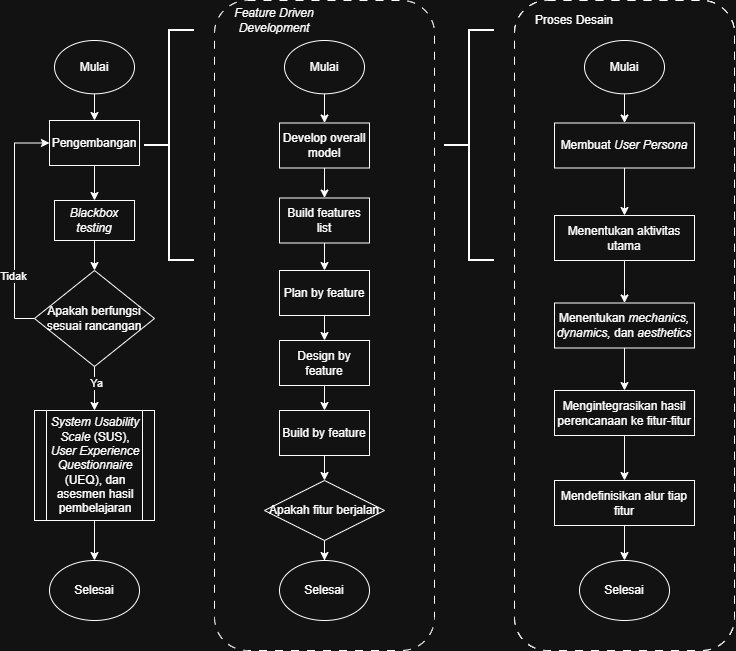
\includegraphics[width=0.7\textwidth]{sample/diagramalur.drawio.png}
	
    \caption{Diagram alur tugas akhir}
    \label{fig:diagram-alur-tugas-akhir}
\end{figure}

\subsection{User Persona}

\subsection{Activity-centered Design}
Metode \textit{Activity-centered Design} digunakan untuk merancang. Aktivitas yang digunakan adalah \textit{fire drill}. \textit{Fire drill} kemudian dibagi menjadi aktivitas-aktivitas yang lebih kecil. Kegiatan-kegiatan tersebut dianalisis dan dijadikan basis untuk tiap level sedemikian sehingga progresi pembelajaran dari level ke level berikutnya dapat dilakukan dengan baik. Hasil perancangan dengan metode \textit{Activity-centered Design} diilustrasikan pada diagram yang ada di Tabel~\ref{tab:scores}.

\begin{table}[h!]
\centering
\caption{Aktivitas Utama}
\begin{tabular}{|p{3cm}|p{12cm}|p{2cm}|}
\hline
\textbf{ID} & \textbf{Aktivitas Utama}  \\ \hline
A-01 & Mempelajari jalur evakuasi saat bencana kebakaran  \\ \hline
A-02 & Mempelajari cara menemukan jalur alternatif saat jalur utama terhalang \\ \hline
A-03 & Mempelajari cara evakuasi aman dengan menghindari asap \\ \hline
A-04 & Mempelajari cara menggunakan APAR saat keadaan darurat dan membuat keputusan dengan cepat  \\ \hline
A-05 & Mempelajari evakuasi yang lebih kompleks dengan menggabungkan A-01 sampai A-04  \\ \hline
\end{tabular}

\label{tab:scores}
\end{table}

% See Table~\ref{tab:scores} for details.


\subsection{Rancangan Permainan dengan kerangka MDA}
Rancangan permainan dapat dijelaskan dengan menggunakan kerangka \textit{Mechanics, Dynamics, and Aesthetics} (MDA). \textit{Mechanics} adalah aturan-aturan yang mengatur permainan, seperti cara bermain, tujuan permainan, dan interaksi antar pemain. \textit{Dynamics} adalah bagaimana mekanika tersebut berinteraksi dengan pemain selama permainan berlangsung, seperti strategi yang muncul dan pengalaman yang dirasakan pemain. \textit{Aesthetics} adalah pengalaman emosional dan estetika yang dirasakan pemain saat bermain, seperti kesenangan, tantangan, dan kepuasan. Rancangan permainan dengan kerangka MDA memastikan bahwa permainan tidak hanya memiliki mekanika yang baik tetapi juga memberikan pengalaman yang menyenangkan dan memuaskan bagi pemain. Kerangka MDA juga menjelaskan hubungan antara fitur permainan, pola perilaku, dan pengalaman yang dihasilkan. Tabel~\ref{tab:kerangka-mda} menunjukkan keterkaitannya secara ringkas.

\begin{table}[h!]
\centering
\caption{Kerangka MDA}
\begin{tabular}{|p{2cm}|p{4cm}|p{4cm}|p{4cm}|}
\hline
\textbf{Fitur} & \textbf{Mekanika} & \textbf{Dinamika} & \textbf{Estetika} \\ \hline
 Mode Pembelajaran dan Mode Permainan & dsds & Pemain mengikuti instruksi dan petunjuk di model belajar dan menguji kemampuan evakusasi di mode permainan  & Rasa penasaran dan aman saat belajar dan   \\ \hline
 Level dan Progresi Kesulitan & dsds & Mempelajari jalur evakuasi saat bencana kebakaran & Mempelajari jalur evakuasi saat bencana kebakaran \\ \hline
Lokomosi dan Interaksi dengan Perangkat Pengontrol Meta Quest 2 & dsds & Mempelajari cara evakuasi aman dengan menghindari asap & Mempelajari jalur evakuasi saat bencana kebakaran \\ \hline
Area Picu (\textit{trigger area}) & dsds & Mempelajari cara menggunakan APAR saat keadaan darurat dan membuat keputusan dengan cepat & Mempelajari jalur evakuasi saat bencana kebakaran  \\ \hline
Muncul (\textit{spawn}) dan Muncul Kembali (\textit{respawn}) & dsds & Mempelajari evakuasi yang lebih kompleks dengan menggabungkan A-01 sampai A-04 & Mempelajari jalur evakuasi saat bencana kebakaran    \\ \hline
\end{tabular}

\label{tab:kerangka-mda}
\end{table}

Dalam permainan FireDrillVR ini, mekanika permainan adalah sebagai berikut.
\begin{enumerate}
	\item \textbf{Mode} \\ FireDrillVR memiliki dua mode, yaitu mode pembelajaran dan mode permainan. Mode pembelajaran memberikan panduan langkah demi langkah evakuasi yang aman pada tiap levelnya, sedangkan mode permainan memungkinkan pemain untuk mempraktikkan apa yang telah mereka pelajari dengan batasan waktu dan tanpa petunjuk.
	\item \textbf{Level} \\ FireDrillVR dikembangkan dengan enam level berbeda: lima level utama dan satu level khusus APAR. Pemain harus menyelesaikan tugas-tugas yang diberikan di setiap level untuk melanjutkan ke level berikutnya. Tiap level memiliki tantangan yang berbeda, seperti menemukan jalur evakuasi, menghindari asap, dan menggunakan APAR. Progresi kesulitan juga meningkat seiring bertambahnya level dengan level terakhir yang menggabungkan semua tantangan dari level sebelumnya dan semakin tinggi levelnya, semakin tinggi lantai yang harus dievakuasi.
	\item \textbf{Lokomosi dan Interaksi} \\ Pemain dapat bergerak di dalam permainan dengan menggunakan perangkat kontroler \textit{Meta Quest 2}. Perangkat kontroler juga digunakan dalam berinteraksi dengan objek-objek di dalam permainan, seperti menggunakan APAR dan menekan tombol teleportasi.
	\item \textbf{Area Picu} \\ Beberapa level memiliki area picu yang akan memicu kejadian tertentu, seperti munculnya asap atau penghalang jalur, saat pemain melewati area tersebut. Area picu ini dirancang untuk meningkatkan tantangan dan memberikan pengalaman yang lebih realistis.
	\item \textbf{Muncul dan Muncul Kembali} \\ Fitur muncul digunakan untuk teleportasi pemain ke lantai lain. Fitur muncul kembali pula digunakan di beberapa level untuk memungkinkan pemain untuk mencoba kembali jika mereka gagal menyelesaikan level. Selain itu, fitur ini juga digunakan untuk mengembalikan pemain ke adegan permainan awal.
\end{enumerate}

\subsection{\textit{Features List}}
\subsection{Linimasa Pengembangan}
\subsection{\textit{Feature Sets}}
\subsubsection{\textit{Feature set} : Memulai permainan}

\subsubsection{\textit{Feature set} : Mempelajari Penggunaan APAR}

\subsubsection{\textit{Feature set} : Mempraktikkan Penggunaan APAR}

\subsubsection{\textit{Feature set} : Evaluasi Pembelajaran}

\subsubsection{\textit{Feature Set} : Hasil Pembelajaran}

\subsection{\textit{Build by Feature}}

\subsection{Pengujian}
\subsection{Analisis Hasil Pengujian}
\section{Etika, Masalah, dan Keterbatasan Penelitian (Opsional)}

Bagian ini membahas pertimbangan etis penelitian dan [potensi] masalah serta
keterbatasannya. Jika menyangkut penelitian dengan makhluk hidup, maka dibutuhkan adanya \textit{ethical clearance}, di bagian ini hal itu akan dibahas. Demikian juga tentang keterbatasan ataupun masalah yang akan timbul.

